% 87-73(87쪽) — 길이 20인 선분 AB 위의 점 P와, AP·BP 를 각각 지름으로 하는 두 원. 스캔 삽화라 TikZ 로 다시 그림.
% 원문에 있는 것만: 두 원 · 선분 AB · 20 을 가리키는 파선 호 · 점 P 와 P가 움직이는 방향 화살표 · 라벨 A, P, B.
% 원문 그림의 비율(큰 원이 작은 원보다 훨씬 크다)만 옮기고 AP·BP 의 값은 적지 않는다.
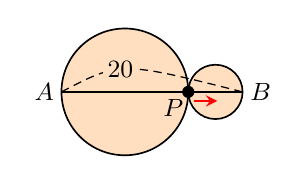
\begin{tikzpicture}[x=0.115cm, y=0.115cm, line width=0.55pt]
  \fill[orange!25] (7,0) circle (7);
  \fill[orange!25] (17,0) circle (3);
  \draw[line width=0.6pt] (7,0) circle (7);
  \draw[line width=0.6pt] (17,0) circle (3);
  \draw[line width=0.6pt] (0,0) -- (20,0);
  \draw[densely dashed, line width=0.45pt] (0,0) .. controls (6.5,3.4) .. (20,0);
  \fill (14,0) circle (2.2pt);
  \draw[->, >=stealth, red, line width=0.8pt] (14.6,-1.0) -- (17.2,-1.0);
  \node[anchor=east, inner sep=2.5pt, font=\small] at (0,0) {$\pt{A}$};
  \node[anchor=north east, inner sep=1.5pt, font=\small] at (14,-0.3) {$\pt{P}$};
  \node[anchor=west, inner sep=2.5pt, font=\small] at (20,0) {$\pt{B}$};
  \node[anchor=south, inner sep=1.5pt, font=\small, fill=orange!25] at (6.5,1.1) {$20$};
\end{tikzpicture}
